\documentclass[a4paper,10pt,oneside]{article}
\usepackage[polutonikogreek,italian]{babel}
\usepackage[utf8x]{inputenc}
\usepackage{amsmath}
\usepackage{amsthm}
\usepackage{amssymb}
\usepackage{amscd}
\usepackage{graphicx}
\usepackage{float}
\usepackage{array}
\usepackage{rotating}
\usepackage[small]{caption}
\usepackage{lscape}
\usepackage{fancybox}
\usepackage{booktabs}
\usepackage[noanswer]{exercise}
\parindent0ex
\renewcommand{\fboxsep}{0.4cm}
\usepackage{hyperref}
\renewcommand{\textfraction}{0.05}
\renewcommand{\topfraction}{0.95}
\renewcommand{\bottomfraction}{0.95}
\renewcommand{\floatpagefraction}{0.35}
\renewcommand{\ExerciseName}{Esercizio}
\renewcommand{\ExerciseListName}{Es}
\setcounter{totalnumber}{5}
\restylefloat{figure}
\begin{document}
\thispagestyle{empty}

\section*{Energia}
\vspace{1cm}


\section*{Conservazione dell'energia meccanica}

Durante questa esperienza verificheremo la conservazione dell'energia meccanica. Il sistema è composto da due masse $M_1$ ed $M_2$ collegate tra loro da una corda inestensibile di peso trascurabile. La massa $M_1$ si trova inizialmente alla quota $h$ mentre la massa $M_2$ è in quiete sulla guidovia. All'istante $t=0$ il sistema viene lasciato libero di muoversi, la massa $M_1$ inizia a cadere e trascina con se la massa $M_2$.

L'energia totale iniziale è data unicamente dall'energia potenziale della massa $M_1$:
\begin{equation}
 E_i=U=M_1gh
\end{equation}
dato che le due masse al tempo $t=0$ sono ferme. Un istante prima che la massa in caduta tocchi il pavimento l'energia totale del sistema è unicamente cinetica dato che la quota è  nulla:
\begin{equation}
 E_f=T_1+T_2=\frac 1 2 M_1v_f^2+\frac 1 2 M_2 v_f^2
\end{equation}
nella relazione precedente $v_f$ rappresenta la velocità delle masse nell'istante precedente a quello in cui $M_1$ raggiunge la quota zero. Per quale motivo le masse hanno la stessa velocità?

\begin{figure}[H]
 \centering
 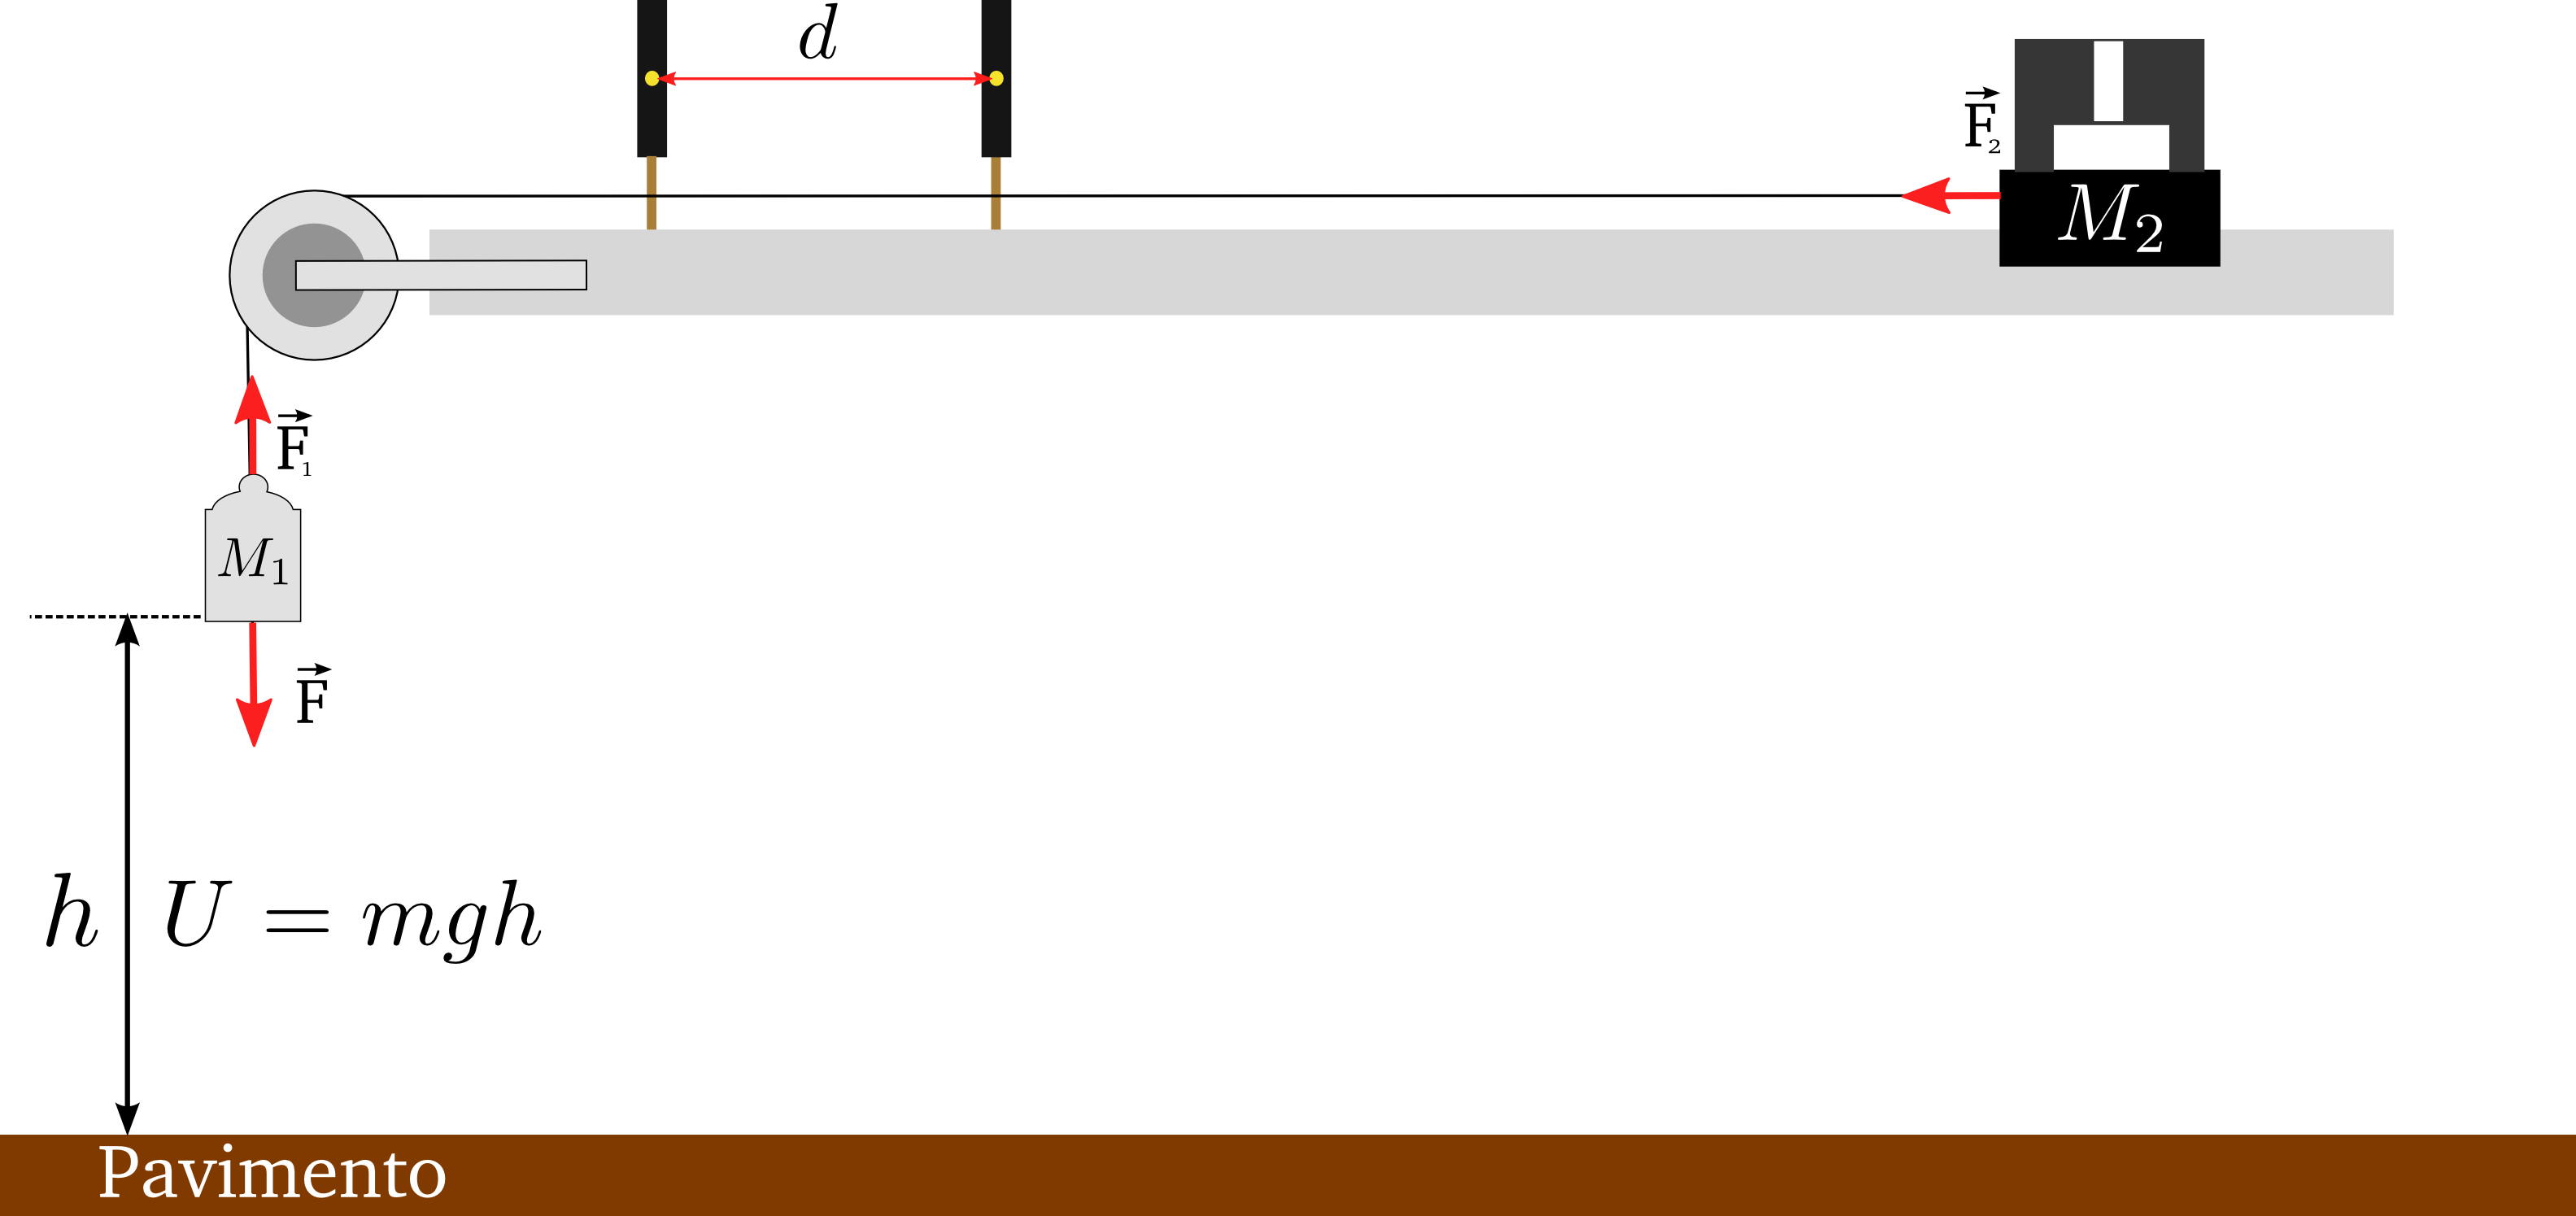
\includegraphics[width=0.8\textwidth]{./immagini/energia_inizio.png}
 % energia_inizio.png: 3167x1495 pixel, 300dpi, 26.81x12.66 cm, bb=0 0 760 359
 \caption{Un istante prima di essere liberato l'energia totale del sistema è unicamente potenziale}
 \label{fig:energia_iniziale}
\end{figure}


Siccome i corpi si muovono all'interno del campo gravitazionale terrestre e nella nostra trattazione gli attriti sono trascurabili, dovrà risultare:
\begin{equation}
 E_i=Ef
\end{equation}
ovvero:
\begin{equation}\label{en_1}
 M_1gh=\frac 1 2 M_1v_f^2+\frac 1 2 M_2 v_f^2
\end{equation}
Per controllare direttamente la veridicità dell'equazione [\ref{en_1}] scriviamo l'energia totale del sistema quando la massa in caduta si trova ad una distanza $x$ dal suolo:
\begin{equation}\label{en_2}
 E=mgx+\frac 1 2 M_1v_x^2+\frac 1 2 M_2 v_x^2
\end{equation}
dove $v_x$ rappresenta la velocità del sistema alla quota $x$. Ricordiamo\footnote{Per i dettagli consultate la nota sulla forze} che l'accelerazione delle due masse in caduta è
\begin{equation}
 a=\frac{M_1}{M_1+M_2}g
\end{equation}


\begin{figure}[H]
 \centering
 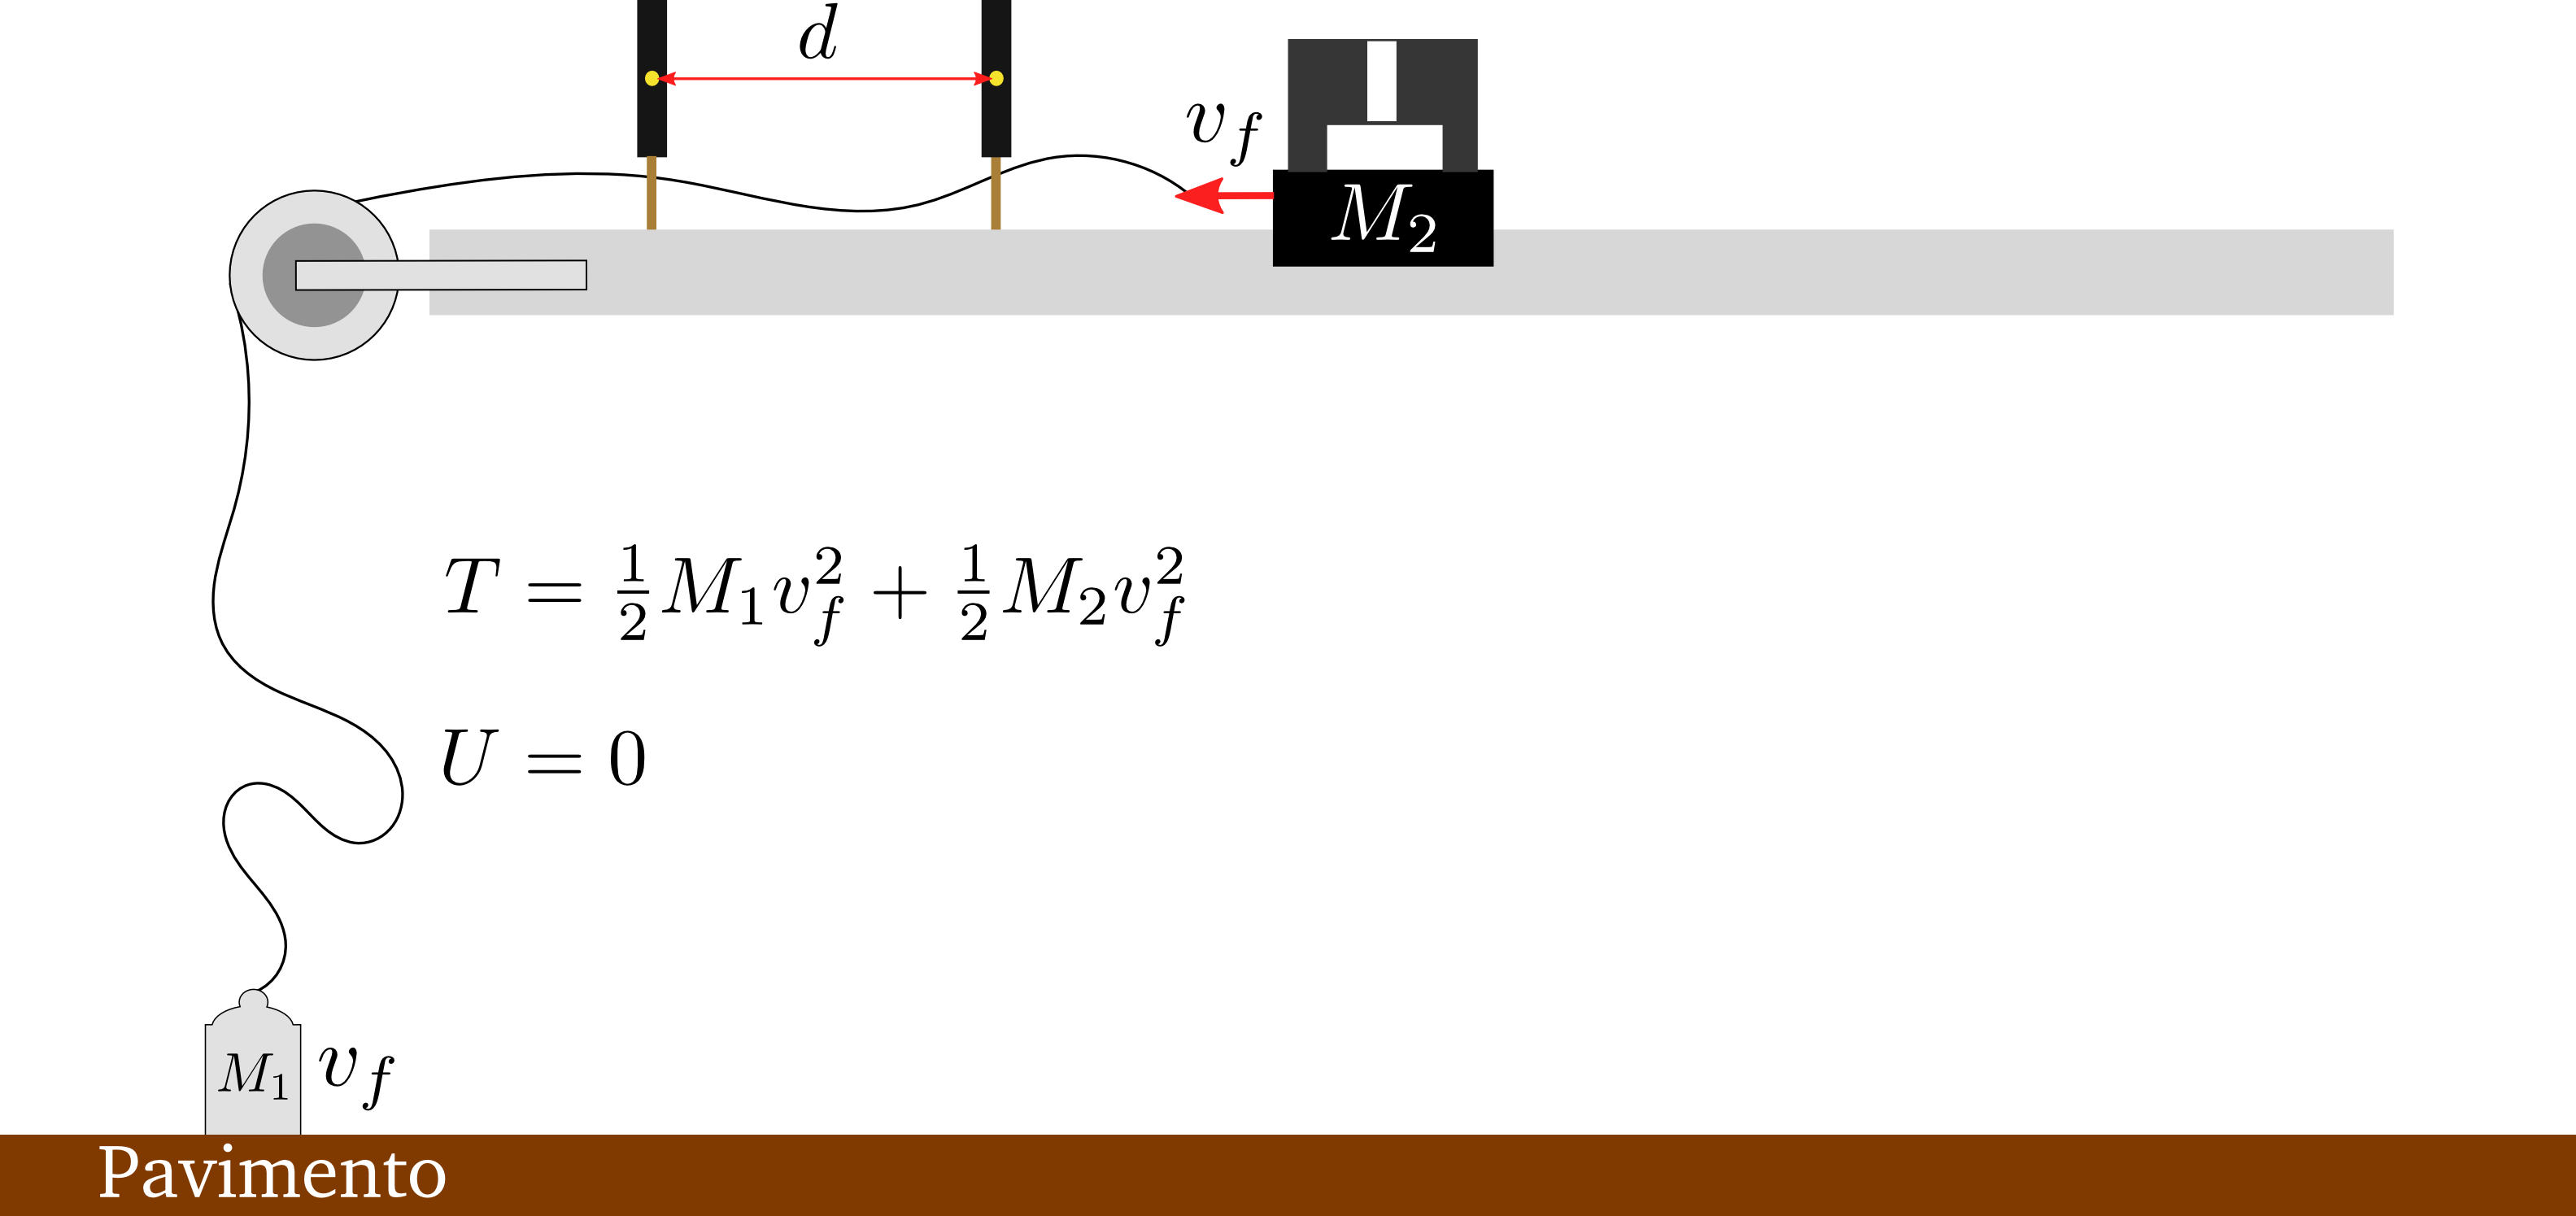
\includegraphics[width=0.8\textwidth]{./immagini/energia_fine.png}
 % energia_fine.png: 3167x1495 pixel, 300dpi, 26.81x12.66 cm, bb=0 0 760 359
 \caption{Un istante prima che la massa  $M_1$ tocchi terra l'energia è totalmente cinetica. Nel momento in cui la massa in caduta si ferma la tensione del filo diventa trascurabile}
 \label{fig:energia_fine}
\end{figure}

Quando il sistema si trova alla quota $x$ le masse si sono spostate di una quantità pari a $h-x$ per cui applicando la nota relazione cinematica:
\begin{equation}
 v_f^2=v_i^2+2a(x-x_0)
\end{equation}
possiamo scrivere:
\begin{equation}\label{vel}
 v_x^2=2\frac{M_1}{M_1+M_2}g(h-x)
\end{equation}
dove si è tenuto conto del fatto che la velocità iniziale è nulla.
Sostituendo  la [\ref{vel}] nella  [\ref{en_2}] otteniamo:
\begin{equation}
 E=mgx+\frac{1}{2}M_12\frac{M_1}{M_1+M_2}g(h-x)+\frac{1}{2}M_22\frac{M_1}{M_1+M_2}g(h-x)
\end{equation}
che con un po' di algebra si trasforma in
\begin{equation}
 E=mgh
\end{equation}
esattamente come ci aspettavamo. Veniamo ora all'esperimento, per la verifica sperimentale della conservazione dell'energia è necessario misurare:
\begin{itemize}
 \item Le due masse $M_1$ ed $M_2$
\item La quota iniziale $h$ della massa $M_1$
\item La velocità finale delle due masse $v_f$
\end{itemize}
per le prime tre quantità utilizzeremo una bilancia ed un metro a nastro, maggiore cura dovrà essere invece utilizzata per la determinazione di $v_f$. Notiamo che quando la massa $M_1$ ha raggiunto il pavimento la massa $M_2$ (il carrello della guidovia) si sta ancora muovendo con la velocità $v_f$ finale del sistema, cosa che continuerà a fare fino alla fine del binario. Siccome nel tratto finale l'accelerazione del carrello è nulla possiamo determinare la velocità utilizzando due fotocellule poste a distanza nota $d$. Le fotocellule sono collegate ad un timer digitale che fornisce il tempo di transito del carrello $\Delta t$, per ottenere la velocità finale sarà dunque sufficiente applicare la definizione di velocità media:
\begin{equation}
 v_f=\frac{d}{\Delta t}
\end{equation}
Ottenuti i dati necessari questi dovranno essere utilizzati per calcolare l'energia potenziale iniziale e l'energia cinetica finale del sistema.


 
\end{document}
